\documentclass[a4paper,12pt]{article}
\usepackage[slovene]{babel}
\usepackage[utf8]{inputenc}
\usepackage{multicol}
\usepackage{fullpage}
\usepackage{guitar}
\usepackage{titlesec}
\usepackage{graphicx}
\setcounter{secnumdepth}{-1} 
\usepackage[absolute]{textpos}
\titleformat{\chapter}{\large\bfseries}{\thesection}{1em}{}
\titleformat{\section}{\Large\bfseries}{\thesection}{1em}{}
\titleformat{\subsection}{\large\bfseries}{\thesection}{1em}{}

\begin{document}
\pagenumbering{Roman}
\begin{titlepage}
\begin{textblock*}{297mm}(-6mm,-0mm)
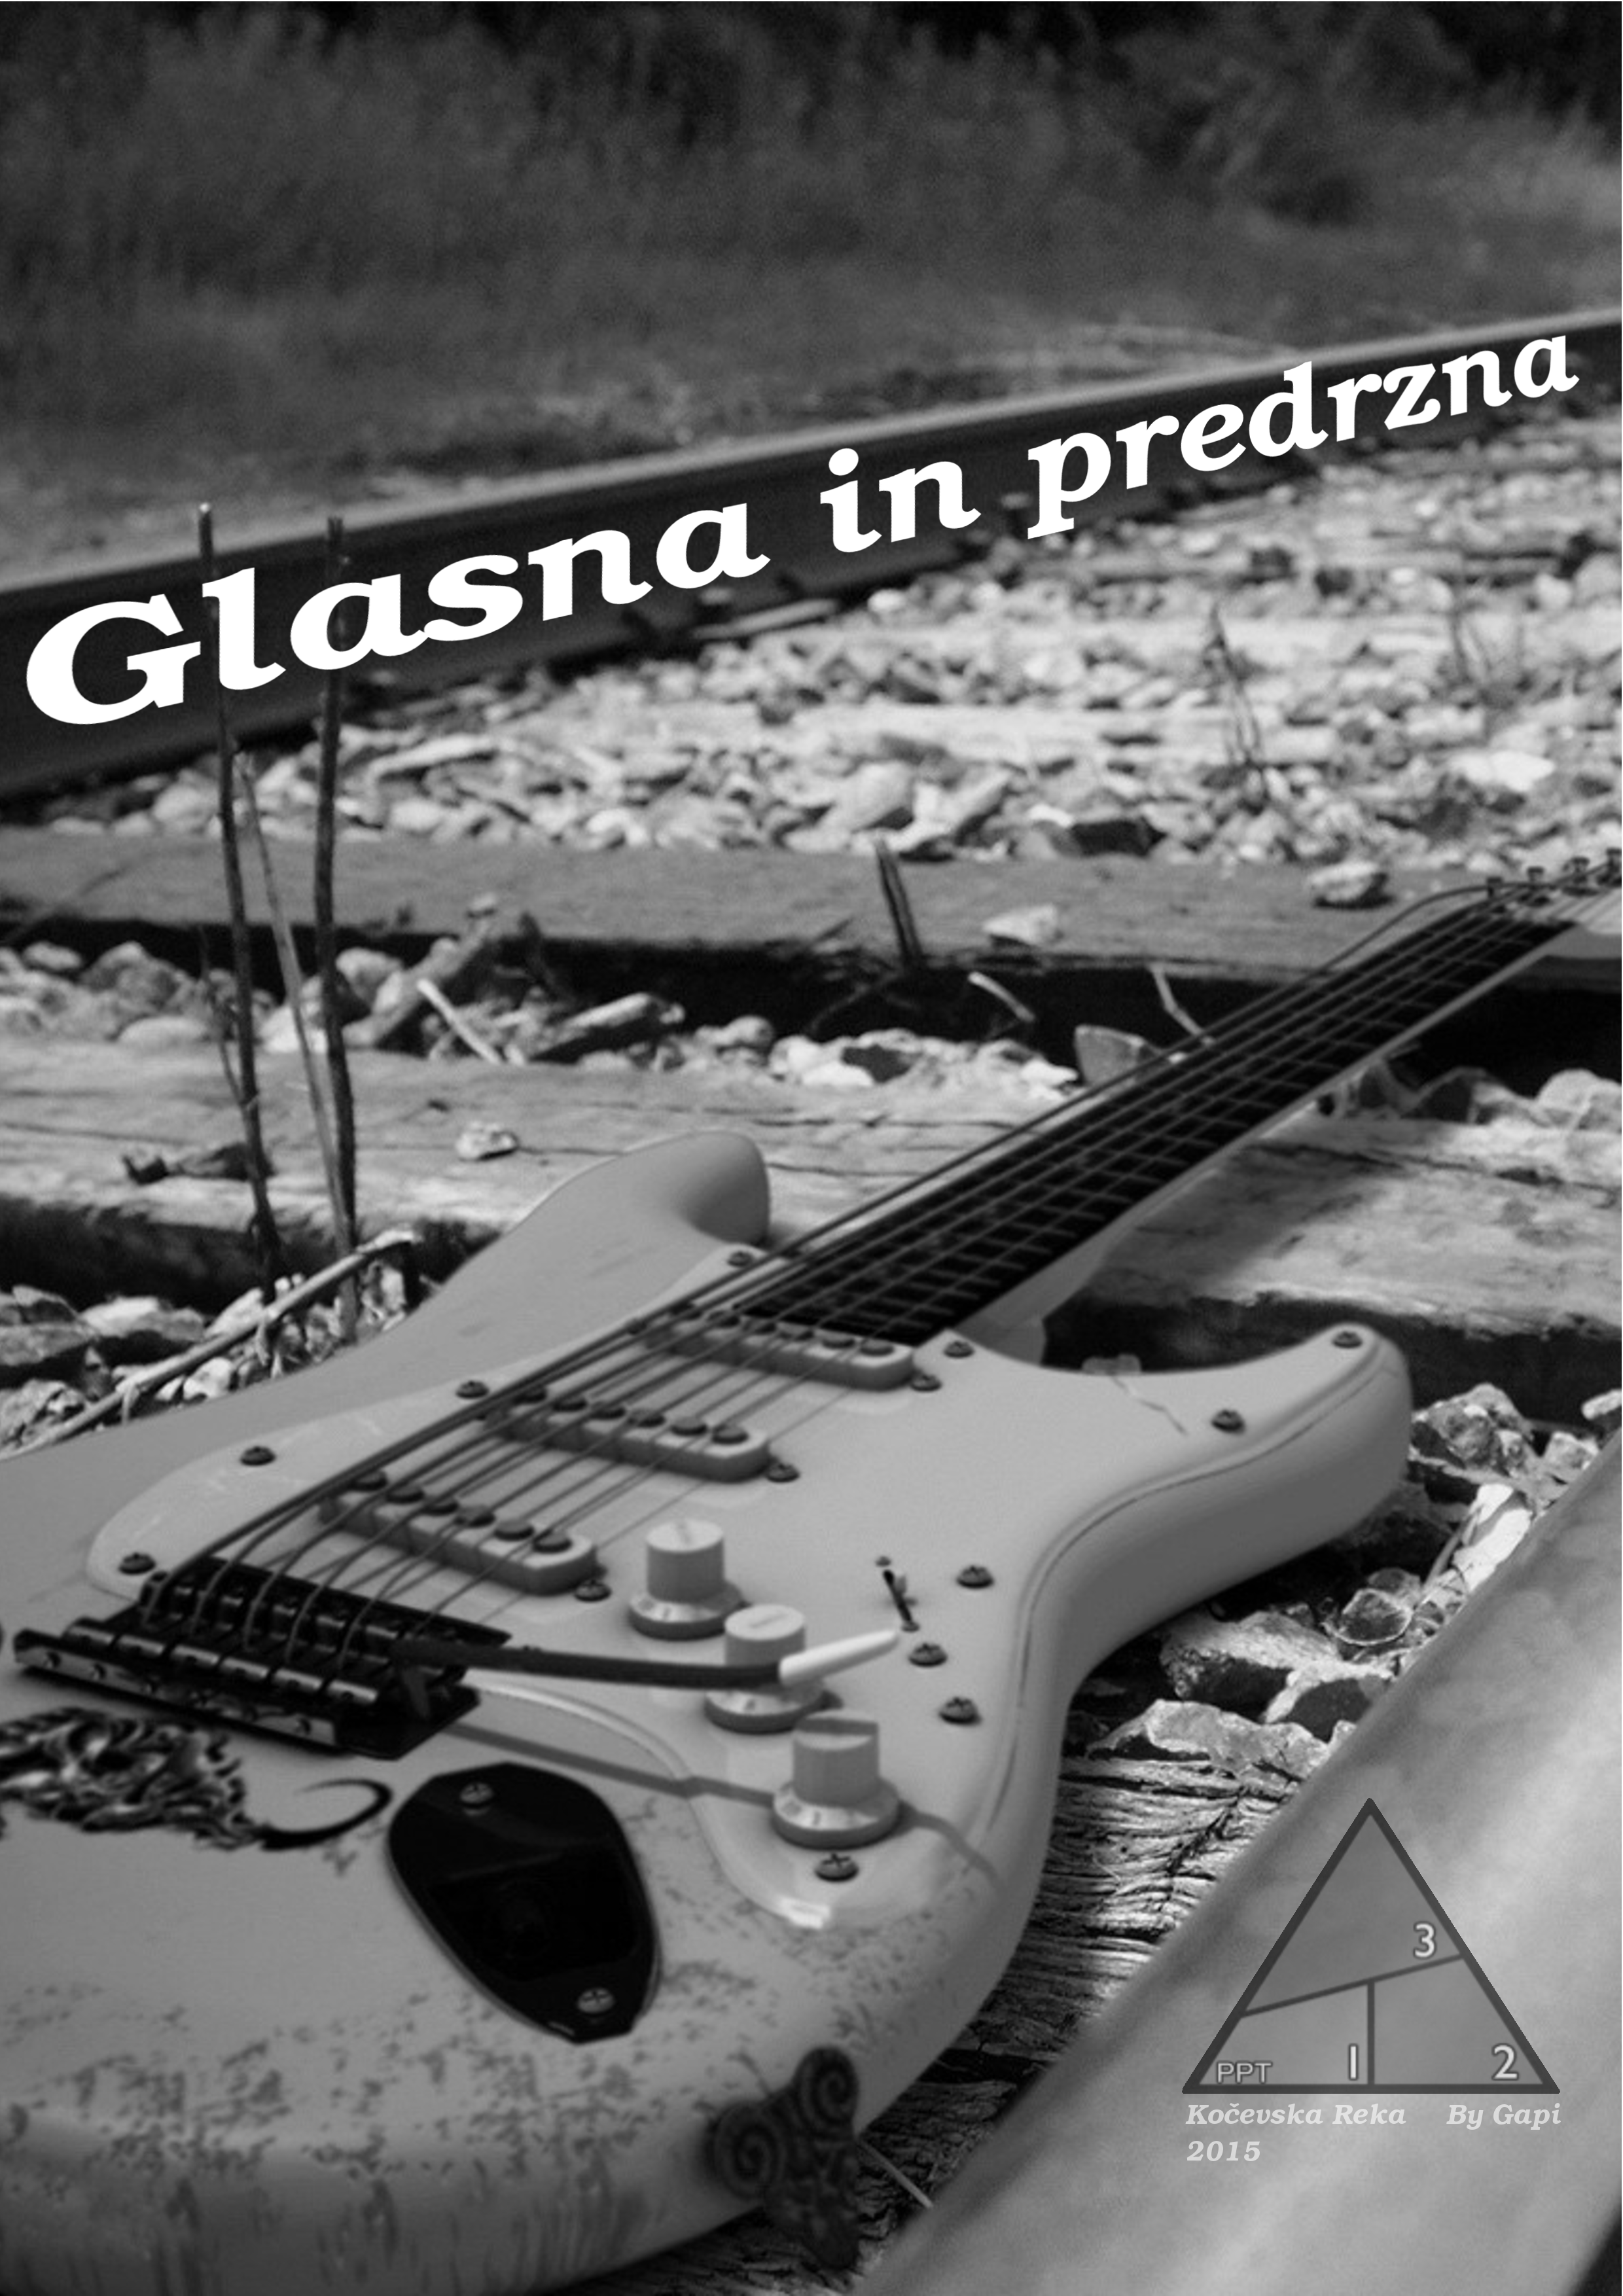
\includegraphics[width=\paperwidth]{img/tpage.png}
\end{textblock*} \
\end{titlepage}
\setlength{\columnseprule}{0.5pt}
\begin{multicols}{2}
\tableofcontents
\end{multicols}
\pagebreak

\setlength{\columnseprule}{0.5pt}
\begin{multicols}{2}
\pagenumbering{arabic}
\section{Akordi}
\begin{guitar}
[A - X02220  Am - X02210]

[B - X13331  Bm - X13321]

[C - X32010  Cm - X35543]  

[D - XX0232  Dm - XX0231] 

[E - 022100  Em - 022000] 

[F - 133211  Fm - 133111]

[G - 320003  Gm - 355333]

[H - X24442  Hm - X24432]


[A7 - X02020  B7 - X13131]

[C7 - X32310  D7 - XX0212]

[E7 - 020100  F7 - 131211]

[G7 - 320001  H7 - X21202]


[Am7 - X02010  Bm7 - X13121]

[Cm7 - X35343  Dm7 - XX0211]

[Em7 - 022030  Fm7 - 131111]

[Gm7 - 353333  Hm7 - X24232]


[C# - X46664  D# - 779997]

[F# - 244322  G# - 466544]


[C#m - X46654  D#m - 779987]

[F#m - 133111  G#m - 466444]


[A6 - X02222  C6 - X055555]

[D6 - X077777 E6 - X099999]


[ASUS2 - X02200]

[ASUS4 - X02230]

[DSUS2 - XX0320] 

[DSUS4 - XX0233]

[ESUS4 - 022200]

[CMAJ7 - X32000]

[FMAJ7 - 103210]

[GMAJ7 - 3X0032]

[DADD4/ADD2 - 554030]

\end{guitar}
\subsection*{Barre akordi}
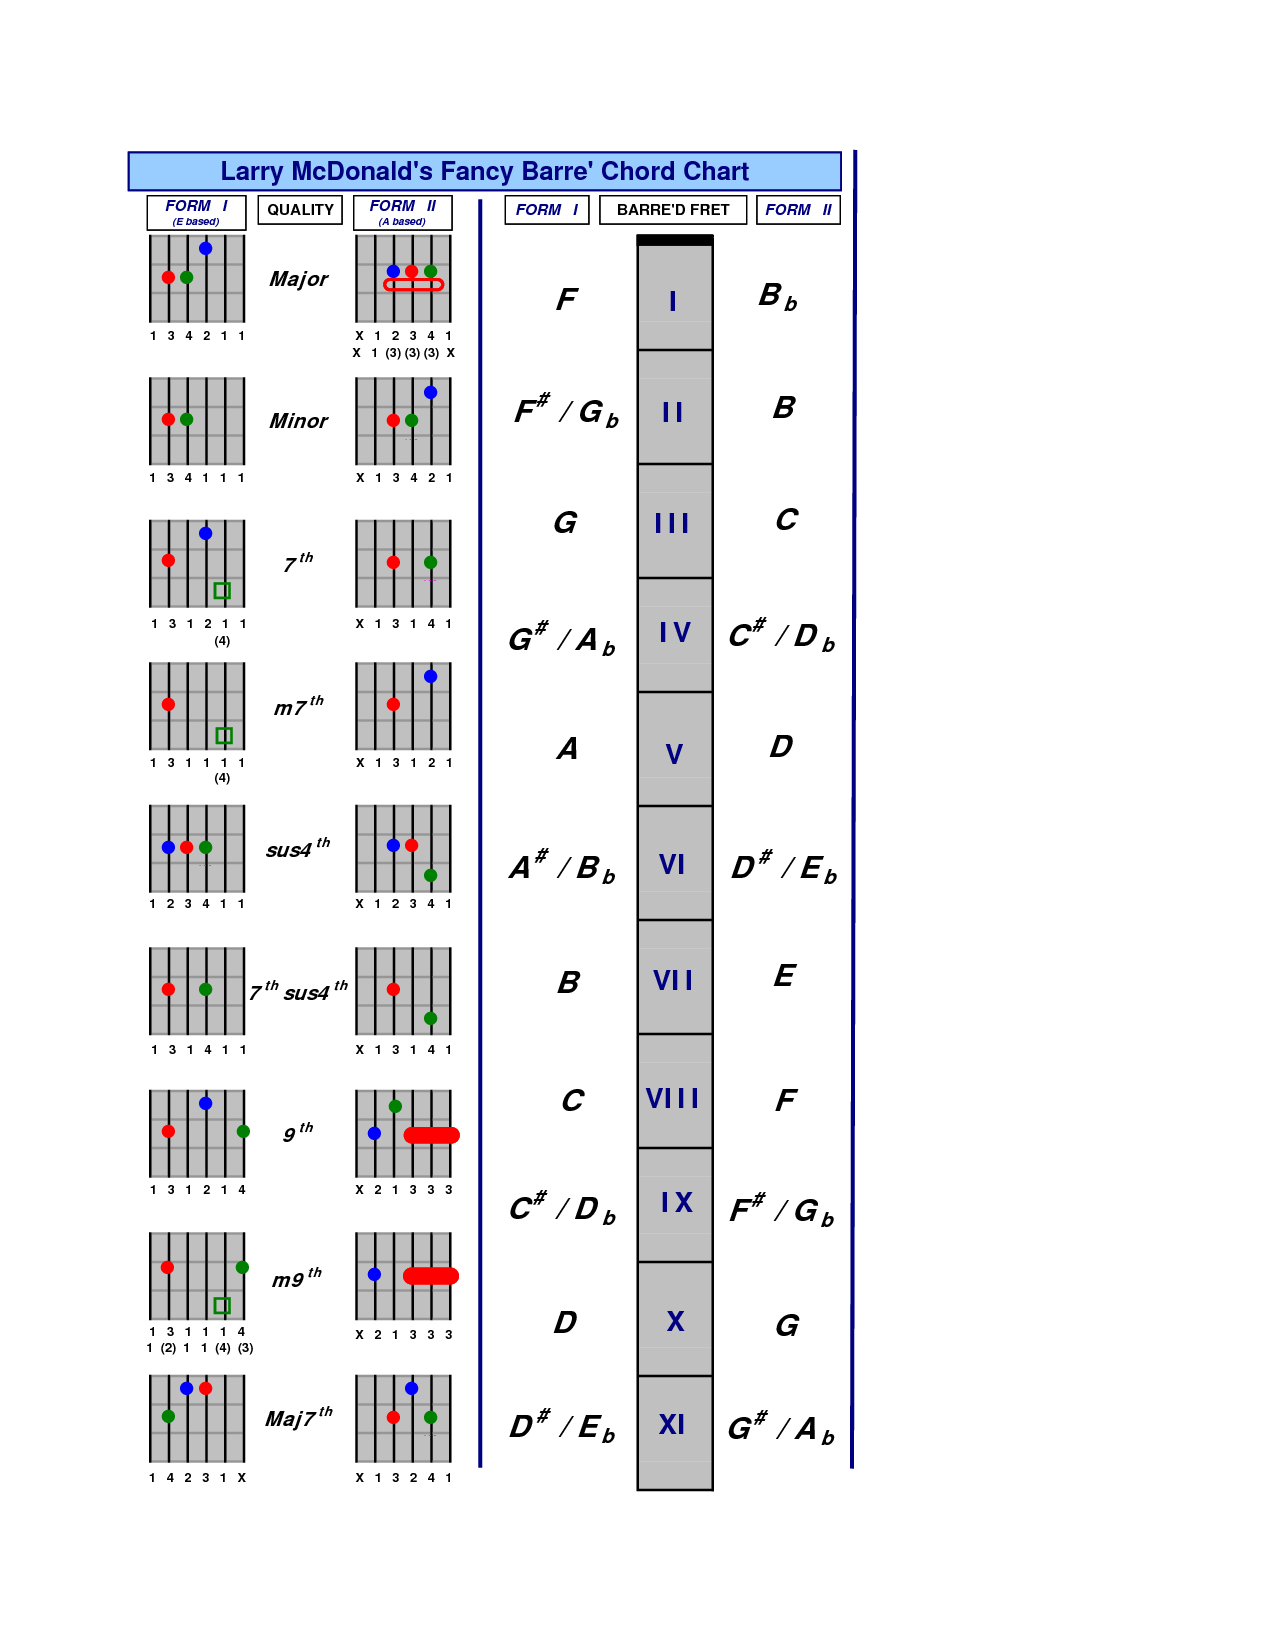
\includegraphics[width=140mm]{img/barre.png}
\clearpage
\section{Jeans generacija}
\subsection*{Neki to vole vruće}
\begin{guitar}
[E]Kažu da je s one strane sad noć,
u toj zemlji, kažu, ponoć će proć'
i da je Johnny skinuo svoj stari [A]jeans.
A ovdje budi se [E]dan.


Oblačim na sebe isti taj jeans
i za Johnnya dižem ruku u vis,
spavaj Johnny, neka te ne plaši [A]mrak.
Mi isti dišemo [E]zrak.



[F#m]Nikada se [D]nismo susreli [F#m]mi,
kilometri [D]su nas dijeli[F#m]li.
Al' smo uvijek [D]isto mislili [E]mi, mi, mi!

Da, mi smo svi [A]jeans generaci[F#m]ja,
i mi smo sad [D]najjača naci[E]ja,
i mi smo i [A]istok i zapad i [F#m]jug,
mi smo to[D]variš, mister i [E]drug.


[E]Oblačim na sebe stari blue jeans
i za tebe dižem ruku u vis,
spavaj mirno, neka te ne plaši [A]mrak.
Mi isti dišemo [E]zrak.


\end{guitar}
\section{Let her go}
\subsection*{Passenger}
\begin{guitar}

[F    G   Am   G (3x)]

[F      G      Am]

Ref.:                                               
Well you only need the [F]light 
when its burning [C]low
Only miss the [G]sun 
when its starts to sn[Am]ow
Only know you [F]love her 
when you let her go [C   G]'
Only know you’ve been [F]high 
when youre feeling low [C]'
Only hate the [G]road 
when youre missin hom[Am]e
Only know you [F]love her 
when youve let her go [C   G]'

And you let her go




[Am     F     G     Em]

[Am    F     G]




[Am]Staring at the bottom of your [F]glass
Hoping one [G]day you will make a dream [Em]last
The dreams come [Am]slow and goes so [F]fast [G]'
You [Am]see her when you close your [F]eyes
Maybe one [G]day you will understand [Em]why
Everything you [Am]touch all it [F]dies [G]'



Ref.



Staring at the ceiling in the dark
Same ol empty feeling in your heart
Love comes slow and it goes so fast
Well you see her when you fall asleep
But to never to touch and never to keep
Because you loved her too much
And you dive too deep



Ref.



Ooooo ooo[F]oo ooo[G]ooo
And you let her go[Am]'
Ooooooo ooo[F]oo ooo[G]oo
And you let her go[Am]'



[F    G]

[Am    F    G]



Ref.

\end{guitar}
\section{Majski šlager}
\subsection*{Kajmak}
\begin{guitar}
[C]Kakor ko se [Am]sneg topi na [F]moji [G]vroči [C]dlani, 
[C]tako se mi to[Am]pi srce ko 
[F]vidim te s kom [G]drugim v Lju[C]bljani. 
[C]In kakor ko žer[Am]javica pade v 
[F]suho [G]travo in jo [C]zge, 
[C]tako me žgejo [Am]tvoje oči ko po 
[F]meni spre[G]hajajajo [C]se.


[F]In…	ne [G]vem zakaj ne [C]grem, 
(paararara pa pa ra ra ra) 
[F]ven saj je [G]maj, saj vendar [C]smem. 
[F]Vendar se mi [G]zdi kot da bi le [C]eni obljubil [Am]se: 
[F]druga ven po[G]vabit me ne [C]sme. 


Daj povej mi: si še sama, 
še kaj misliš name? 
A ti je ostal še del srca, 
ki si ga shranila zame? 
Ali že kdo drug pobral je vse, 
kar nekoč bilo je moje?
Ali ti je pustil vsaj stvari, 
ki jaz sem pustil, da so le tvoje? 


In, nevem zakaj... 


[F]Uuu uuu [G]uuuu ne, ne [C]vem... 
[F]Uuu uuu [G]uuuu zakaj ne [C]grem... 
[F]Uuu uuu [G]uuuu [C]ven, saj je vendar [Am]maj... 
[F]Uuu uuu [G]uuuu mesec, ko se [C]sme... 

\end{guitar}
\section{Moving on}
\subsection*{Melissa Lara Clissold}
\begin{guitar}
[G D Am D G]

[G]Fell in love, fell for [D]you
[Am]Didn't quite work out
[D]The way I had it [G]planned

Took my chances yeah I tried
Wore my heart on my sleeve
Just like every other time

Now I've crashed and I've burned,
Burning is a thing
I've learnt to do quite well

And I've set myself on fire
It's the only thing
That makes me feel alive

[G]Moving [D]on.... [Am D]
[G]Moving [D]on...  [Am D]
[D]On my feet a[G]gain
\end{guitar}
\section{Rad te imam Ivanka}
\subsection*{Kit-art}
\begin{guitar}
A* - 055000
E* - 077000


[A*]Ulice [E*]so p[A*]raz[E*]ne,
[C6]hiše brez [D6]zivljenja, brez od[A]prt[G]ih [E]vrat,
[A*]usta [E*]brez [A*]nasme[E*]ha,
[C6]ljubezen se [D6]izgublja v meg[A]le[G]ni [E]dan.



[G]Pa čeprav danes [D]je še en[A] tu[G]roben [E]dan.
[G]Pa čeprav mene [D]deklica še ne pozna.
Rad te imam Ivanka.



Sanje brez uspeha,
ljubezen hoče vzeti tudi naju dva.
Vzemi mojo roko in zjutraj soncu reči
srečna sva.



Pa čeprav...

\end{guitar}
\section{Terca na tišinu}
\subsection*{Silente}
\begin{guitar}
[C#m]Ne pustaj ni [A]glasa
ja cu na to slozit [E]tercu
prosit dok ne prista[G#]nes
ja cu pozvati [C#m]ljude
ti se pobrini o [A]vinu
prvi svat da nema [E]pjesme
samo terca na ti[G#]sinu
samo terca na ti[C#m]sinu



[C#m H E A G# 2x]



[C#m]Ti vladaj [H]zrakom
ja cu vladati [E]zemljom [A  G#]
[C#m]nadjemo se [H]negdje u sre[E]dini [A  G#]
[C#m]nadjemo se [H]gdje se nadju
[E]tvoje noci i [A]moje [G#]zore
[C#m]nadjemo se kako [H]kazu
[E]nije nebo, a [A]nije ni [G#]more



Ne puštaj mi glasa...


Ja svjetim kao mlad 
u meni istok počiva
priznajem kriv sam za nered u tvojim očima
u tvojim ruskim piscima trežiš meni dostojna
ma sve ti čitam u pjegama, pjegama
pjegama kao zvijezdama


Ne puštaj mi glasa...


Ti spavaj nebom ja ću divljati svijetom
nađemo se negdje u sredini
ma nađemo se gdje se nađu
tvoji oblaci i moje gore
nađemo se već si mašu
tvoje pjege i moje bore


Ne puštaj mi glasa... 2x

\end{guitar}
\end{multicols}
\clearpage
\clearpage
\null
\vfill
\center

\includegraphics[width=100px]{img/licence.png}

Pesmarica je zaščitena z licenco CC-BY-NC-SA. Vse pesmi so delo in last avtorjev. Morebitne napake in predloge sporočite na pesmarica.info@gmail.com 

Izvorna koda (LaTeX) ter PDF sta dostopna na https://github.com/gztproject/Pesmarica
\end{document}
